\documentclass[12pt]{article}%

% Packages to be used
\usepackage[a4paper, top=2.5cm, bottom=2.5cm, left=2.2cm, right=2.2cm]%
{geometry}
\usepackage{xcolor}
\usepackage{blindtext}
\usepackage{mathtools}
\usepackage{algorithmic}
\usepackage{graphicx}
\usepackage{tabularx}
\usepackage{authblk}

% Some new colors defined
\definecolor{aliceblue}{rgb}{0.94, 0.97, 1.0}
\definecolor{cream}{rgb}{1.0, 0.99, 0.82}

%title section
\title{Assignment 1}
\author[1]{Atharva Swami\\
\texttt{190010008@iitdh.ac.in}}
\affil[1]{CSE, IIT Dharwad}
\date{\today}

%document begins here
\begin{document}
\maketitle

\tableofcontents
\listoffigures
\listoftables

\newpage
%table section
\begin{table}
    \centering
    \begin{tabularx}{0.9\textwidth} { 
  | >{\raggedright\arraybackslash}X 
  | >{\centering\arraybackslash}X 
  | >{\raggedleft\arraybackslash}X | }
 \hline
 CS201 & Data Structures and Algorithms \\
 \hline
 CS203  & Discrete Structures  \\
\hline
CS213  & Software Systems Lab  \\
\hline
CS211  & Data Structures and Algorithms Lab  \\
\hline
EE201  & Data Analysis  \\
\hline
HS201  & Economics  \\
\hline
\end{tabularx}
    \caption{III Sem Courses}
    \label{tab:my_label}
\end{table}

% Figures
\begin{figure}
    \centering
    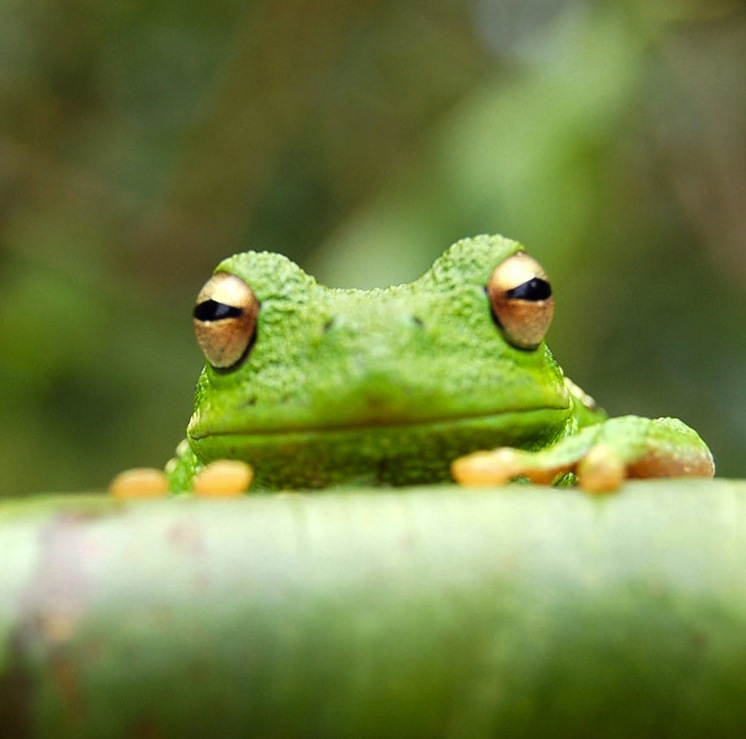
\includegraphics[width=0.5\textwidth]{frog.jpg}
    \caption{Frog}
    \label{fig:my_label}
\end{figure}

%maths section starts here
\section{Mathematics} \label{sec:maths}
{Albert Einstein's famous mass-energy equation is $E=m{c}^2$}\\
To know more about this equation refer\cite{bodanis2000mc2}.\\
{Photoelectric Energy Formula $\Rightarrow$ $$ E = hv - \phi $$}\\
Refer \cite{smoluchowski1941anisotropy} for more on this formula.\\
{Basic numbered equation $\Rightarrow 1 + 1 = 2$}\\
Energy of light is
\begin{align} \label{eq:light}
E &= mc^2\\
&= \frac{(mc)^2}{m}\\
&= \frac{p^2}{m}
\end{align}
Took reference from \cite{irodov1991problems}.\\
Identity matrix $\Rightarrow$
$I = \begin{bmatrix}
       1 & 0 & 0 \\[0.3em]
       0 & 1 & 0 \\[0.3em]
       0 & 0 & 1
     \end{bmatrix}$\\
\\
\\Square root 
$\Rightarrow \sqrt{1+x^2+x^4}$\\
Average of n number is an array(a) 
$\Rightarrow 
\frac{
\displaystyle\sum_{i=1}^{n} a_i}{n}$\\
\\Integrals 
$\Rightarrow \int_V xy^2z^3 d(V) = \iiint_V xd(x) y^2d(y) z^3d(z) $\\
\\Nested brackets 
$\Rightarrow a + b + \Bigg( c + d +\bigg( e + \Big( f + \big( g \big) \Big) \bigg) \Bigg) $
\\Fraction $\Rightarrow \frac{\frac{1}{a}+\frac{1}{b}+\frac{1}{c}}{a+b+c}$\\

%cross references
\section{Cross-Referencing}
In Table~\ref{tab:my_label}, we have showed the courses.\\
In Figure~\ref{fig:my_label}, we display a frog.\\
In Section~\ref{sec:maths}, we display all the Maths Equations and Expressions.\\
In Equation~\ref{eq:light},we have showed the Energy of light.\\
In Section~\ref{sec:lists},we have displayed different kinds of Lists.\\

%This section has different font styles
\section{Font Styles}
\textbf{This is a bold font}\\
\textit{This is an italic font}\\
\underline{This is an underlined font}\\
\emph{This text is emphasized}\\
\texttt{This text is teletype}\\
\textsc{This is small capitals}\\
\uppercase{This is uppercase}\\
\lowercase{This is lowercase}\\
\textrm{This is roman font}\\
Refer \cite{hoenig1998tex} for more fonts.\\

%This is color section
\section{Color}
{\color{red} This is a text in red color} \\
{\colorbox{cyan}{This text has a cyan color text background}}\\
This page color is yellow\\
\pagecolor{yellow}

\newpage
\section{Lists} \label{sec:lists}
\begin{enumerate}
     \item Types of Lists
     \item 1st level item
       \begin{enumerate}
       \item This is enumerated
       \item 2nd level item
         \begin{itemize}
            \item This is itemized
            \item 3rd level item
            \begin{description}
                \item[option1] This is description
                \item[option2] 4th level item
            \end{description}
       \end{itemize}
     \end{enumerate}
   \end{enumerate}

\pagecolor{white}
%quick sort
\section{Quick Sort Algorithm}
\begin{algorithmic}
\STATE quickSort($arr[], low, high$)
{
    \IF{$low < high$}
    {
        \STATE $pi$ = partition($arr, low, high$)\;
        \STATE quickSort($arr, low, pi - 1$)\; 
        \STATE quickSort($arr, pi + 1, high$)\; 
    } \ENDIF
}
\STATE partition ($arr[], low, high$)
{
    \STATE $pivot = arr[high]$\;  
    \STATE $i = (low - 1)$\;
    \STATE $j \gets low $\;
    \WHILE{$j \leq high- 1$} 
    {
        \IF{$arr[j] < pivot$}
        {
            \STATE $i++$\;    
            \STATE swap ($arr[i],arr[j]$)\;
        } \ENDIF
        \STATE $j++$\;
    } \ENDWHILE
    \STATE swap ($arr[i + 1],arr[high]$)\;
    \STATE \RETURN ($i + 1$)
}
\\Refer \cite{10.1145/1498698.1564500} to know more about quick sort.\\

\newpage
%references
\bibliographystyle{plain}
\bibliography{references.bib}


\end{algorithmic}

\end{document}


